% \begin{toappendix}

\section{Checklist}

\subsection{Broader Impacts}
Our work pushes the quantization of large language models into the 2 bits per weight regime.
Our aim is to drive foundational research on theoretical and empirical aspects of quantization.
The ultimate goal is to enable more powerful LLMs to run more efficiently.
However our work is unaware to what ends those LLMs are used.


\subsection{Limitations}
The adaptive rounding~\cite{nagel2020up} proxy objective considers each layer in isolation; it remains to be seen what other computationally tractable proxies could improve quantization.
For example quantization methods do exist which consider interactions between layers, but so far have been too computationally expensive to be applied to the largest open LLMS.


\subsection{Experiments, Reproducibility}
Our code is included in the Supplement.
See the included README for instructions on how to reproduce the various experiments, including random seeds.
The code also downloads all datasets used to quantize or evaluate the models.


\section{Additional Method Clarifications}\label{suppExtraMethod}
\subsection{Subsection~\ref{secAddHeur} (Incoherence-Based Heuristics)}
Line~\ref{alg1rescale_a} diagonally rescales $W$ and $H$ to minimize $\ell(\hat W) \approx \trace{H} \|W\|_F^2$, effectively trading off the spectrum of these matrices to find a minimum.
Note to minimize $\trace{ D^{-1} H D^{-1} } \|W D\|_F^2 = (\sum_{i=1}^n H_{ii} / D_i^2) (\sum_{i=1}^n D_i^2 \|W_i\|^2)$ implies that $D_i = \sqrt{H_{ii} / \|W_i\|}$.
Motivated by the incoherence of $W$, Line~\ref{alg1reducedquant} computes the quantization range depending on the spectrum $\|W\|_F$, instead of the typical $\max_{i,j} |W_{ij}|$.
The parameter $\rho$ controls the quantization range; we tune it and find that a value of 2.4 works well across all our experiments.
We use $\rho=2.4$ consistently across all experiments.
Our full QuIP procedure is described in Algorithm~\ref{algQuIP}, which contains calls to the pre- and post-processing sub-steps in Algorithms~\ref{algQuIPpre} and~\ref{algQuIPpost}.




\subsection{Subsection~\ref{secAddHeur} (Greedy Updates)}

In this subsection, we describe the ``greedy local search'' method mentioned in the main body of the paper in more detail.
The basic idea is to iterate over coordinates of the weights in the same order as the initial quantization method, modifying each weight in turn---but still restricting it to be a representable quantized value---so as to minimize the proxy loss while keeping the other weights fixed.
These greedy updates amount to coordinate descent on the proxy loss, but restricted to the quantization grid.
Greedy updates can be performed after any initial quantization method, or as a standalone method.
When performed after an initial quantization method, greedy local search is a \emph{descent method} because the individual weight updates cannot increase the loss, but when performed alone, these greedy updates are not a descent method because the initial point ($\hat W = W)$ is not feasible because it contains unquantized values that are off the representable quantization grid.
Concretely, a greedy update of weight $(i,j)$ to the grid $\{0,1,\ldots,2^b - 1\}$ does the following, where $\ell$ is the proxy loss:
\[
    \hat W_{ij} \gets \arg \min_{z \in \{0,1,\ldots,2^b - 1\}} \ell(\hat W - e_i e_j^T \hat W_{ij} + e_i e_j^T z).
\]
(Note that $\hat W - e_i e_j^T \hat W_{ij} + e_i e_j^T z$ is the result of setting the $(i,j)$th entry of $\hat W$ to $z$.)
A full pass of greedy updates constitutes $mn$ of these updates performed in the same order as LDLQ.
This algorithm is very simple, since it is just greedy coordinate descent. In the rest of this subsection, we will give a bit more intuition about this method by showing how this greedy algorithm falls within our framework of adaptive rounding with linear feedback.

An application of greedy local search as a single-pass stand-alone method falls under our Adaptive Rounding with Linear Feedback framework, with the linear feedback set to $U = (H \odot M) \diag{H}^{-1}$, where $M$ is the strictly upper triangular mask and $\odot$ denotes the Hadamard (entrywise) product, as we will derive below.
For ease of explanation consider a single (row) weight vector $w \in \R^{1 \times n}$.
When looking only at column $j$, the proxy loss from setting $\hat w_j$ to $z$ is
\begin{align*}
    \ell(\hat w - \hat w e_j e_j^T + z e_j^T) 
    &= 
    (\hat w - w) H (\hat w - w)^T
    +
    2 (z e_j^T - \hat w e_j e_j^T) H (\hat w - w)^T
    \\&\hspace{4em}+
    (z e_j^T - \hat w e_j e_j^T) H (z e_j^T - \hat w e_j e_j^T)^T.
\end{align*}
This is just a quadratic function in $z$, and so its minimum value on the grid $\{0, 1, \ldots, 2^{b} - 1\}$ will just be its minimum value on $\R$ rounded to that grid.
To find this minimum over $\R$, we differentiate to minimize, yielding
\[
    0
    =
    2 e_j^T H (\hat w - w)^T
    +
    2 e_j^T H (z e_j^T - \hat w e_j e_j^T)^T,
\]
and solving for $z$,
\begin{equation}
    \label{eqnGreedyZ}
    z
    =
    -
    \frac{
        (\hat w - \hat w e_j e_j^T - w) H e_j
    }{
        e_j^T H e_j
    }
    =
    \hat w e_j
    -
    \frac{
        (\hat w - w) H e_j
    }{
        e_j^T H e_j
    }.
\end{equation}
Since when we use greedy local search as a stand-alone method, we have not updated $\hat w_j$ yet, at this point $\hat w e_j = w e_j$, and so
this means that a single step of greedy updates looks like
\[
    \hat w e_j \gets \mathcal{Q}\left( w e_j - (\hat w - w) \frac{
        H e_j
    }{
        e_j^T H e_j
    } \right)
\]
for $\mathcal{Q}$ referring to nearest rounding with the necessary clamping. Since $\hat w - w$ is zero for all entries following the $j$th one, this is equivalent to 
\[
    \hat w e_j \gets \mathcal{Q}( w e_j - (\hat w - w) U e_j )
\]
where $U$ is set as $U = (H \odot M) \diag{H}^{-1}$ as above.
This shows how this single-pass version of greedy updates fits into our adaptive rounding with linear feedback framework.


\begin{algorithm}[t]
\caption{Greedy Updates: A Single Pass}\label{algSuppGreedy}
\begin{algorithmic}[1]
\Require $b \in \mathbb{N}$, $H \in \mathbb{R}^{n \times n}$ SPD, weights $W \in \R^{m \times n}$, initial guess $\tilde W$
\State $\hat W \gets \tilde W$
\State $U \gets (H \odot M) \diag{H}^{-1}$ \Comment{$M$ is the strictly upper triangular mask}
\State $V \gets W - (\tilde W - W) (H \odot M^T) \operatorname{diag}(H)^{-1}$ \Comment{can skip if $\tilde W = W$ by setting $V \gets W$}
\State \textbf{for} $k \in \{1, \dots, n\}$ \textbf{do}  
$\hat W_k \gets \operatorname{clamp}(\round_{\operatorname{near}}( V_k + (W - \hat W) U_k ), 0, 2^b-1)$
\State \Return $\hat W$ 
\end{algorithmic}
\end{algorithm}

Analyzing greedy local search as a post-processing pass is a bit more difficult, but we will see that it can also be written as something like adaptive rounding with linear feedback.
Suppose that we do a pass of greedy updates, but our quantized weights start at an initial value $\hat w = \tilde w$ already quantized from some previous method (e.g. LDLQ).
Returning to (\ref{eqnGreedyZ}), since we haven't updated $\hat w_j$ yet, we'll have
\[
    z
    =
    \tilde w e_j
    -
    \frac{
        (\hat w - w) H e_j
    }{
        e_j^T H e_j
    }.
\]
Now, all the entries of $\hat w $ which come \emph{after} $j$ are still the ones from $\tilde w$. This means that we can split this up as
\[
    z
    =
    w e_j
    -
    \frac{
        (\hat w - w)_{:,1:(j-1)} H_{1:(j-1),j}
        +
        (\tilde w - w)_{:,(j+1):n} H_{(j+1):n,j}
    }{
        e_j^T H e_j
    }
\]
where the first part of this sum comes from the entries which we \emph{may} have already updated during this pass, the second comes from the entries which are still equal to their initial values in $\tilde w$, and the case of $w_j$ is handled specially, cancelling it with the $\tilde w e_j$ term.
We can write this more compactly in matrix form as
\[
    z
    =
    w e_j
    -
    \frac{
        (\hat w - w) (H \odot M) e_j
        +
        (\tilde w - w) (H \odot M^T) e_j
    }{
        e_j^T H e_j
    },
\]
where $M$ is the strictly upper triangular mask and $\odot$ is elementwise multiplication. This yields a final quantization step of
\[
    \hat w e_j \gets \mathcal{Q}\left( w e_j - (\tilde w - w) \frac{
        (H \odot M^T) e_j
    }{
        e_j^T H e_j
    }
    - 
    (\hat w - w) \frac{
        H e_j
    }{
        e_j^T H e_j
    } \right).
\]
So, more generally, if we define $U$ as above, and set
\[
    V = W - (\tilde W - W) (H \odot M^T) \operatorname{diag}(H)^{-1},
\]
we can write a single pass of greedy updates in matrix form as
\[
    \tilde W \gets \mathcal{Q}( V + (W - \hat W) U ),
\]
which is very close to our rounding with linear feedback form, albeit with the difference that here $V$ is in place of $W$. 
This is made explicit in the included Greedy Updates Algorithm.


We can use this algorithm both as a whole quantization method (by setting $\tilde W = W$) or as a post-processing step (by setting $\tilde W$ to the output of some other initial quantization algorithm, such as LDLQ). When we do use it as a post-processing step, we typically run multiple passes of greedy updates (e.g. 10 passes): this involves passing the output of the greedy updates algorithm back in as the input guess $\tilde W$ to another run of the greedy updates algorithm, and repeating this multiple times.

\section{Additional Experimental Descriptions and Results}\label{suppAddResults}
\subsection{Subsections~\ref{secLDLopt} and~\ref{secIncoherOpt} (Empirical Properties of $H$ Across OPT-125m to 2.7b)}
\begin{table}[t]
\centering
\begin{tabular}{cc|ccc}
\multirow{2}{*}{Model}\Bstrut & 
\multirow{2}{*}{Processing} & 
Absolute & Approximate &
\multirow{2}{*}{$\trace{D} / \trace{H}$} \\
& & Fractional Rank & Fractional Rank & \\
\hline
\multirow{2}{*}{OPT-125m}\Tstrut & Baseline & 
0.926 ($\pm$0.172) &
0.112 ($\pm$0.127) &
0.540 ($\pm$0.093) \\
& Incoherent\Bstrut & 
0.910 ($\pm$0.196) &
0.124 ($\pm$0.141) &
0.534 ($\pm$0.094) \\
\multirow{2}{*}{OPT-350m} & Baseline\Tstrut &
0.916 ($\pm$0.180) &
0.047 ($\pm$0.032) &
0.445 ($\pm$0.100) \\
& Incoherent\Bstrut &
0.908 ($\pm$0.183) &
0.059 ($\pm$0.062) &
0.440 ($\pm$0.106) \\
\multirow{2}{*}{OPT-1.3b} & Baseline\Tstrut &
0.541 ($\pm$0.404) &
0.020 ($\pm$0.023) &
0.399 ($\pm$0.187) \\
& Incoherent\Bstrut &
0.543 ($\pm$0.405) &
0.028 ($\pm$0.023) &
0.393 ($\pm$0.189) \\
\multirow{2}{*}{OPT-2.7b} & Baseline\Tstrut &
0.426 ($\pm$0.413) &
0.019 ($\pm$0.015) &
0.384 ($\pm$0.206) \\
& Incoherent\Bstrut &
0.427 ($\pm$0.415) &
0.018 ($\pm$0.025) &
0.375 ($\pm$0.205) \\
\Bstrut
\end{tabular}
\caption{
We compute $H$ in each layer of a given model, and compute the following summary statistics.
%
$\trace{D}/\trace{H}$ decreases as the mode size increases, though the variance also increases.
We compute the fraction of nonzero eigenvalues (i.e. absolute), and the fraction of eigenvalues $> 0.01 \cdot \max(\eig{H})$ (i.e. approximate).
The fractional rank is $k / n$ for a rank-$k$ matrix $H$ with dimension $n$.
Mean and standard deviations are computed across layers in a model.
}
\label{tabsuppHSummary}
\end{table}

\paragraph{Interpreting the exact proxy loss of LDLQ and nearest rounding by empirically comparing $\trace{D}$ vs $\trace{H}$.}
Theorem~\ref{thmLDLopt} gives the average-case proxy loss for LDLQ in terms of $\trace{D}$, where $D$ is from the LDL decomposition of $H$.
Lemma~\ref{lemNearStochProxyH} gives the average-case proxy loss for standard nearest rounding in terms of $\trace{H}$.
We know that LDLQ is better in practice, but comparing these equations is difficult because we need to reason about $\trace{D}$ vs $\trace{H}$.
Our paper resolves this difficulty by deriving bounds on the proxy loss for LDLQ in terms of the spectrum of $H$ (with and without incoherence).
However we also perform a quick empirical check: if $\trace{D} \ll \trace{H}$, then our theory explains the empirical superiority of LDLQ over nearest rounding (at least on these models).
Table~\ref{tabsuppHSummary} gives the ratio $\trace{D} / \trace{H}$ across all layers for OPTQ models 125m to 2.7b; the mean value is always less than $0.55$, and it falls as the model gets larger. 

\paragraph{$H$ is approximately low-rank.}
Subsection~\ref{secIncoherOpt} plotted the normalized eigenvalues of $H$ from 3 randomly chosen layers in OPT-2.7b.
Table~\ref{tabsuppHSummary} gives much more evidence that $H$ is consistently approximately low-rank.
Across each model, we calculate the absolute and approximate fractional rank of $H$ across all layers in OPT models 125m to 2.7b (explanations in the caption).
The approximate fractional rank decreases as model size increases; for OPT-2.7b the fractional rank is $\approx 0.02 (\pm 0.02)$.


\subsection{Subsection~\ref{secOPTQequiv} (Empirical Verification of OPTQ Equivalence)}
We share a python script in the supplementary code which empirically verifies that our implementation of LDLQ produces quantized values exactly matching OPTQ's~\cite{frantar2023gptq} implementation.
While we prove the equivalence between LDLQ and OPTQ's respective algorithm statements, empirically comparing ours and \citet{frantar2023gptq}'s code ensures that the respective implementations are sufficiently close to their algorithmic statements.
Therefore we can be sure that LDLQ and OPTQ are equivalent in their implementation.


\definecolor{codegreen}{rgb}{0,0.6,0}
\definecolor{codegray}{rgb}{0.5,0.5,0.5}
\definecolor{codepurple}{rgb}{0.58,0,0.82}
\definecolor{backcolour}{rgb}{0.95,0.95,0.92}

\lstdefinestyle{mystyle}{
    backgroundcolor=\color{backcolour},   
    commentstyle=\color{codegreen},
    keywordstyle=\color{violet},
    numberstyle=\tiny\color{codegray},
    stringstyle=\color{codepurple},
    basicstyle=\ttfamily\footnotesize,
    breakatwhitespace=false,         
    breaklines=true,                 
    captionpos=b,                    
    keepspaces=true,                 
    numbers=left,                    
    numbersep=5pt,                  
    showspaces=false,                
    showstringspaces=false,
    showtabs=false,                  
    tabsize=2,
    xleftmargin=12pt
}

\lstset{style=mystyle}

\subsection{Subsection~\ref{secFiniteGrid} (Empirical Verification of LDLQ/OPTQ Finite Grid Counterexample)}
The following code constructs a weight matrix $W$ and Hessian matrix $H$ where OPTQ performs worse than nearest when rounding to a finite grid.
\begin{lstlisting}[language=Python]
import torch 
def make_counterexample(n, d, c=0.01):
    H = torch.ones(n,n) + torch.eye(n)
    H[n-1,n-1] = 1.0
    H[0,1:(n-1)] += 2 * c
    H[1:(n-1),0] += 2 * c
    H[0,n-1] += c
    H[n-1,0] += c
    H[0,0] += 4 * c + n * (c**2)
    W = 0.499 * torch.ones(d,n) + 0.002 * (torch.arange(n) % 2)
    return W, H
\end{lstlisting}
The intuition behind this counterexample is as follows: 
we want to quantize many coordinates in $W$ in such a way that OPTQ excepts there to be a very large error correction to quantize the last entry.
However, the finite grid restricts this large error correction.
Note that we can achieve this poor OPTQ behavior with {\texttt c=0}, but here nearest rounding also does poorly.
We make a small perturbation ({\texttt c=0.01}) to make OPTQ round in the wrong direction, but not nearest.



\subsection{Additional Details on the Experimental Setup and Computational Resources}
We run experiments on a university cluster managed by a Slurm workload manager which has GPUs with up to 48GB of memory, though larger GPUs are only required for some methods on larger model sizes.
Note we use the LAMBADA OpenAI version.
When Greedy updates are used, we perform 10 passes over the weights in the same order as LDLQ and OPTQ, except for 5 passes on OPT-30b and OPT-66b.
For the incoherence-based quantization range, we tune the parameter $\rho$ and find that a value of 2.4 works well across all model sizes and quantization methods. We use this value for all our experiments.


\subsection{Section~\ref{secExp} 
(Main Results on Additional Evaluations)
}
\begin{figure}[t]
\centering
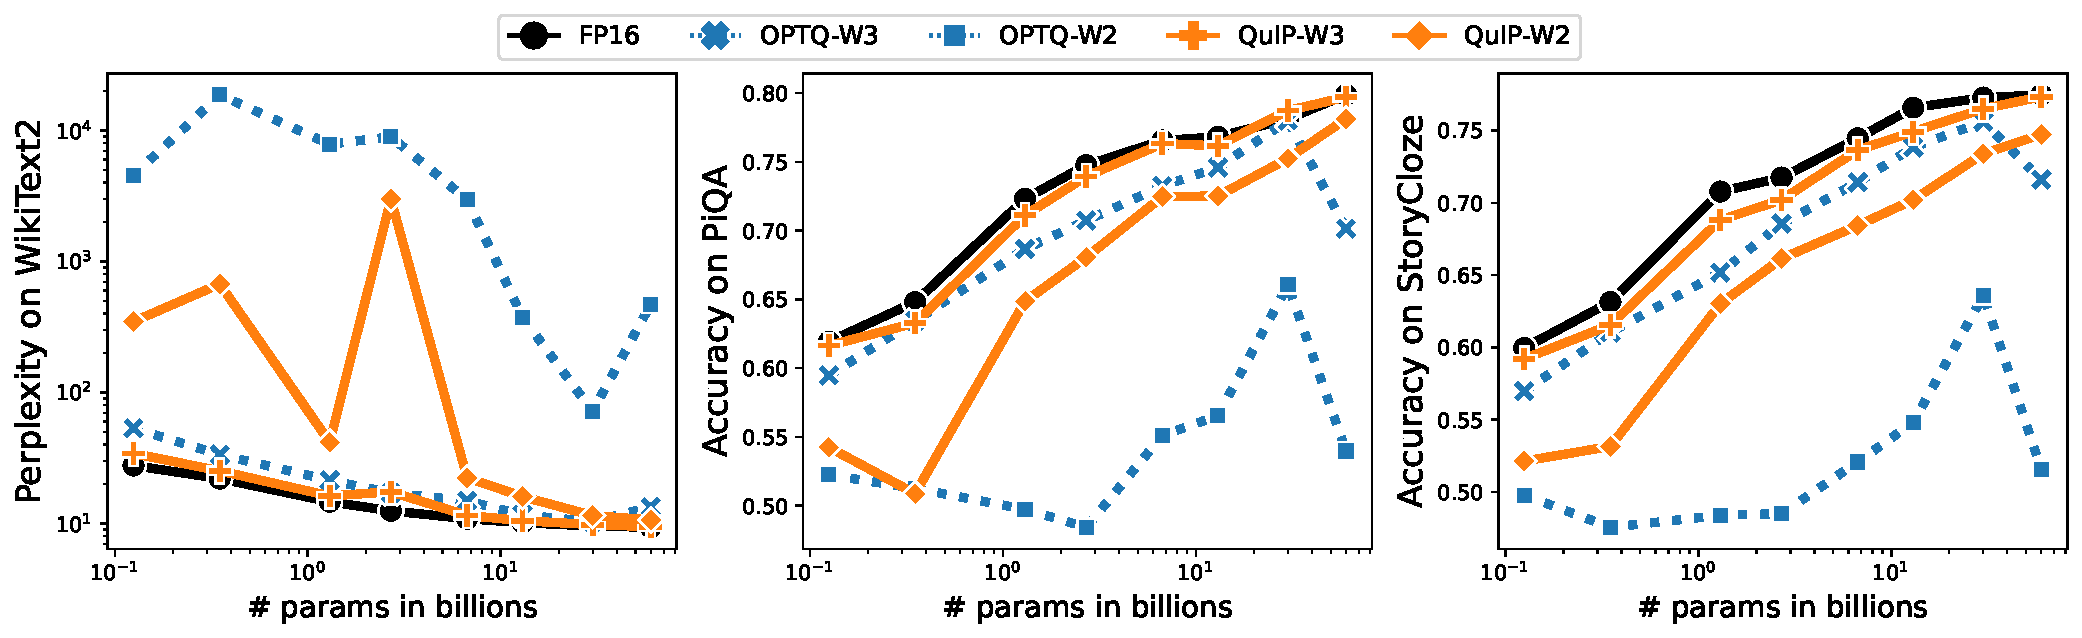
\includegraphics[width=1\linewidth]{figures/main_plot_supp_newcolor.pdf}
\caption{
Quantizing OPT models up to 66B parameters.
Additional evaluation tasks shown here in the Supplement.
Our method QuIP is the first PTQ procedure to achieve good quantization at 2 bits per weight, across a variety of model sizes and evaluation tasks.
Note the drop in performance for OPTQ on OPT-66B is documented in their paper.
}
\label{figSuppMain}
\end{figure}
Figure~\ref{figSuppMain} shows additional results for QuIP and OPTQ on  WikiText2, PiQA, and StoryCloze when quantizing to 2 and 3 bits per weight. 
The insights about our method QuIP remain the same after viewing these additional results: QuIP is the first PTQ procedure to achieve good quantization at two bits per weight, across a variety of LLM sizes and evaluation tasks.
We evaluate on OPT models (up to 30B); 4-bit quantization works equally well for both methods.
QuIP is superior to OPTQ across model sizes and evaluation tasks here.

On WikiText2 2-bit quantization, note that the trend in perplexity for QuIP mirrors the trend in perplexity for OPTQ.
We run OPTQ's~\cite{frantar2023gptq} implementation, though they did not report 2-bit results at this model size.
Because OPTQ is equivalent to QuIP's quantization sub-procedure,
it thus makes sense that worse performance in the quantization sub-procedure could result in worse overall performance.
OPTQ increases perplexity when going from OPT-1.3b to OPT-2.7b. 
QuIP's perplexity also increases from OPT-1.3b to OPT-2.7b, and is unusually higher than the adjacent OPT-1.3b and OPT-6.7b models.
However QuIP still beats OPTQ in this setting.
Our observations about OPTQ and QuIP on WikiText2 and OPT-2.7b were consistent across multiple independent runs.


\subsection{Section~\ref{secExp} (All Methods, All Model Sizes, All Bit Weights, All Evaluation Tasks)}
Tables~\ref{tabSuppAllOPT30b}-\ref{tabSuppAllOPT125m} 
provide results on all combinations of the following: methods, model sizes (OPT 125m-30b), bit weights(4,3,2), and evaluation tasks.
Across our extensive array of experiments, we see that incoherence processing always enables a step function change in quantization at 2 bits.

\input{tables/all_opt30b}
\input{tables/all_opt13b}
\input{tables/all_opt6.7b}
\input{tables/all_opt2.7b}
\input{tables/all_opt1.3b}
\input{tables/all_opt350m}
\input{tables/all_opt125m}

\newpage
\newpage
\newpage
\newpage


\subsection{Section~\ref{secExp} (Evaluating the Effectiveness of the Proxy Objective)}
\begin{table}[h!]
\centering
\begin{tabular}{c|cccc}
WBits\Bstrut & LDLQ/OPTQ & LDLQ-RG & Greedy & Near \\
\hline
4\Tstrut &
104.09 &
105.23 &
120.74 &
301.18
\\
3 &
529.53 &
475.25 &
537.98 &
1,308.05
\\
2 &
2,554.89 &
2,291.02 &
2,587.17 &
5,971.69
\\
\end{tabular}
\caption{
Weighted average of proxy Loss $\trace{ (\hat W - W) H (\hat W - W)^T }$ over OPT models 125m to 2.7b.
Proxy is averaged over models normalized by their model dimension (768, 1024, 2048, 2560) respectively, to ensure proxy loss is comparable across models of different size.
We do not conduct any processing in the proxy evaluation.
Trends in the proxy largely reflect end-to-end results: at 2 bits OPTQ, LDLQ-RG, and Greedy are roughly equivalent, and all do better than nearest.
}
\label{tabSuppProxy}
\end{table}
In Table~\ref{tabSuppProxy} we show the proxy loss of the four quantization methods we evaluate, evaluated over OPT models 125m to 2.7b.
The proxy is averaged over models proxy losses normalized by their model dimension; we use $H$ matrices computed as a result of OPTQ and nearest rounding.
We do not conduct any processing in the proxy evaluation; this is an evaluation of the rounding methods only.
Trends in the proxy reflect end-to-end results. 
OPTQ/LDLQ, LDLQ-RG, and Greedy are roughly equivalent at 2 bits, and do better than Nearest.


\subsection{Section~\ref{secExp} (Evaluating Unbiased Rounding in LDLQ/OPTQ)}
\begin{table}[h!]
\centering
\begin{tabular}{c|cccc|cccc}
& \multicolumn{8}{c}{AVERAGE(Perplexity Unbiased - Perplexity Biased) on Wiki, PTB, C4 ($\downarrow$)}\Bstrut \\
\hline
& \multicolumn{4}{c}{\underline{Incoherence Processing}} &
\multicolumn{4}{c}{\underline{Baseline Processing}}\Tstrut\Bstrut \\
WBits\Tstrut\Bstrut & 125m & 350m & 1.3b & 2.7b & 125m & 350m & 1.3b & 2.7b \\
\hline
4\Tstrut &
1.23 & 0.73 & 0.79 & 0.19 & 27.81 & 5.58 & 1.62 & 0.87
\\
3 &
13.26 & 7.79 & 2.14 & 4.66 & 880.4 & 499.4 & 28.63 & 16.23
\\
2\Bstrut & 
2,501 & 18,732 & 544.8 & 2,251 & 241.3 & 17,945 & 4,831 & 3,798
\\
\end{tabular}
\caption{
Average perplexity difference (i.e. unbiased - biased) for LDLQ/OPTQ on WikiText2, PTB, and C4.
That is, we can run LDLQ with the $\round$ subroutine as stochastic rounding, instead of nearest.
The average difference is positive, meaning that unbiased rounding performs worse than biased (i.e. nearest) across OPT models 125m to 2.7b.
Note the magnitude of the gap increases at lower bits.
}
\label{tabSuppUnbiased}
\end{table}

Note in our formulation for Adaptive Rounding with Linear feedback, the $\round$ subroutine could be biased, or unbiased.
It is typical to perform biased rounding in practice; here we investigate if there is any benefit to switching to unbiased rounding schemes.
Table~\ref{tabSuppUnbiased} computes the average perplexity difference (i.e. $\operatorname{unbiased} - \operatorname{biased}$) for LDLQ/OPTQ on WikiText2, PTB, and C4.
That is, we run LDLQ with the $\round$ subroutine as stochastic rounding, instead of nearest.
The average difference is positive (and large for 2 and 3 bits), meaning that unbiased rounding performs worse than biased (i.e. nearest) across OPT models 125m to 2.7b.
These results indicate that in practice, we want to stick with biased rounding schemes.

\subsection{Section~\ref{secExp} (Evaluating Algorithm~\ref{alg:qcvx} Which Accounts for Clamping)}
\begin{table}[h!]
\centering
\begin{tabular}{cc|ccc|ccc}
& & 
\multicolumn{3}{c}{\underline{Incoherence Processing (ours)}}\Bstrut &
\multicolumn{3}{c}{\underline{Baseline Processing}} \\
Model & WBits\Tstrut\Bstrut & Wiki & PTB & C4 & Wiki & PTB & C4 \\
\hline
\multirow{3}{*}{OPT-1.3b}
& 4\Tstrut &
16.54 & 22.12 & 17.58 &
15.43 & 21.92 & 16.80 \\
& 3 &
18.27 & 23.96 & 18.66 &
20.45 & 28.86 & 20.68 \\
& 2\Bstrut &
38.13 & 51.78 & 31.09 &
6,438.75 & 6,099.27 & 2,057.71 \\
\hline
\multirow{3}{*}{OPT-350m}
& 4\Tstrut &
23.19 & 32.55 & 23.48 &
23.71 & 33.73 & 24.29 \\
& 3 &
25.54 & 36.74 & 25.52 &
33.01 & 45.15 & 30.09 \\
& 2\Bstrut &
286.71 & 367.26 & 144.08 &
8,006.22 & 7,445.70 & 2,317.18 \\
\hline
\multirow{3}{*}{OPT-125m}
& 4\Tstrut &
32.04 & 44.56 & 29.08 &
32.59 & 41.95 & 28.67 \\
& 3 &
40.66 & 51.90 & 32.91 &
50.73 & 74.14 & 41.04 \\
& 2\Bstrut &
1,649.83 & 240.86 & 136.55 &
3,714.11 & 4,703.76 & 1,848.72 \\
\end{tabular}
\caption{
Quantizing OPT models using Algorithm~\ref{alg:qcvx} evaluated on WikiText2, PTB, and C4.
At 2 bits and incoherence processing, we see improvements over LDLQ and LDLQ-RG on OPT-125m and OPT-350m, but diminishing improvements on OPT-1.3b.
Due to Algorithm~\ref{alg:qcvx}'s relatively equivalent performance relative to QuIP at OPT-1.3b, and due to this algorithm's increased computational cost, we decide not to user it.
}
\label{tabSuppADMM}
\end{table}

Table~\ref{tabSuppADMM} shows results from using Algorithm~\ref{alg:qcvx} to quantize OPT models 125m to 1.3b, with incoherence processing and baseline processing.
At 2 bits and incoherence processing, we observe modest improvements over QuIP in terms of perplexity on OPT models 125m and 350m.
However, at the larger OPT-1.3b QuIP beats Algorithm~\ref{alg:qcvx} on 2/3 language generation tasks.
In addition, Algorithm~\ref{alg:qcvx} is computationally more work to run.
Therefore we decide not to use it.

Another observation: in practice, we don't seem to encounter constructions of $W$ and $H$ that are bad for LDLQ/OPTQ. 
Therefore this ``clamping'' issue seems to not be an issue in practice, especially as model size increases.